\section{Middlebox Implementation}
\label{sec:netshaper-middlebox-implementation}

While it is possible to apply NetShaper framework's approach at any network layer, we chose to develop the system as an L4 (Transport Layer) proxy.
This enables the system to be easily deployable, entirely in userspace and without requiring any superuser privileges. 
Developing NetShaper at L2 (Data Link Layer) or L3 (Network Layer) would require the deployer to either have the ability to modify the OS kernel or deploy some form of kernel bypass.

\begin{figure}[!htb]
    \centering
    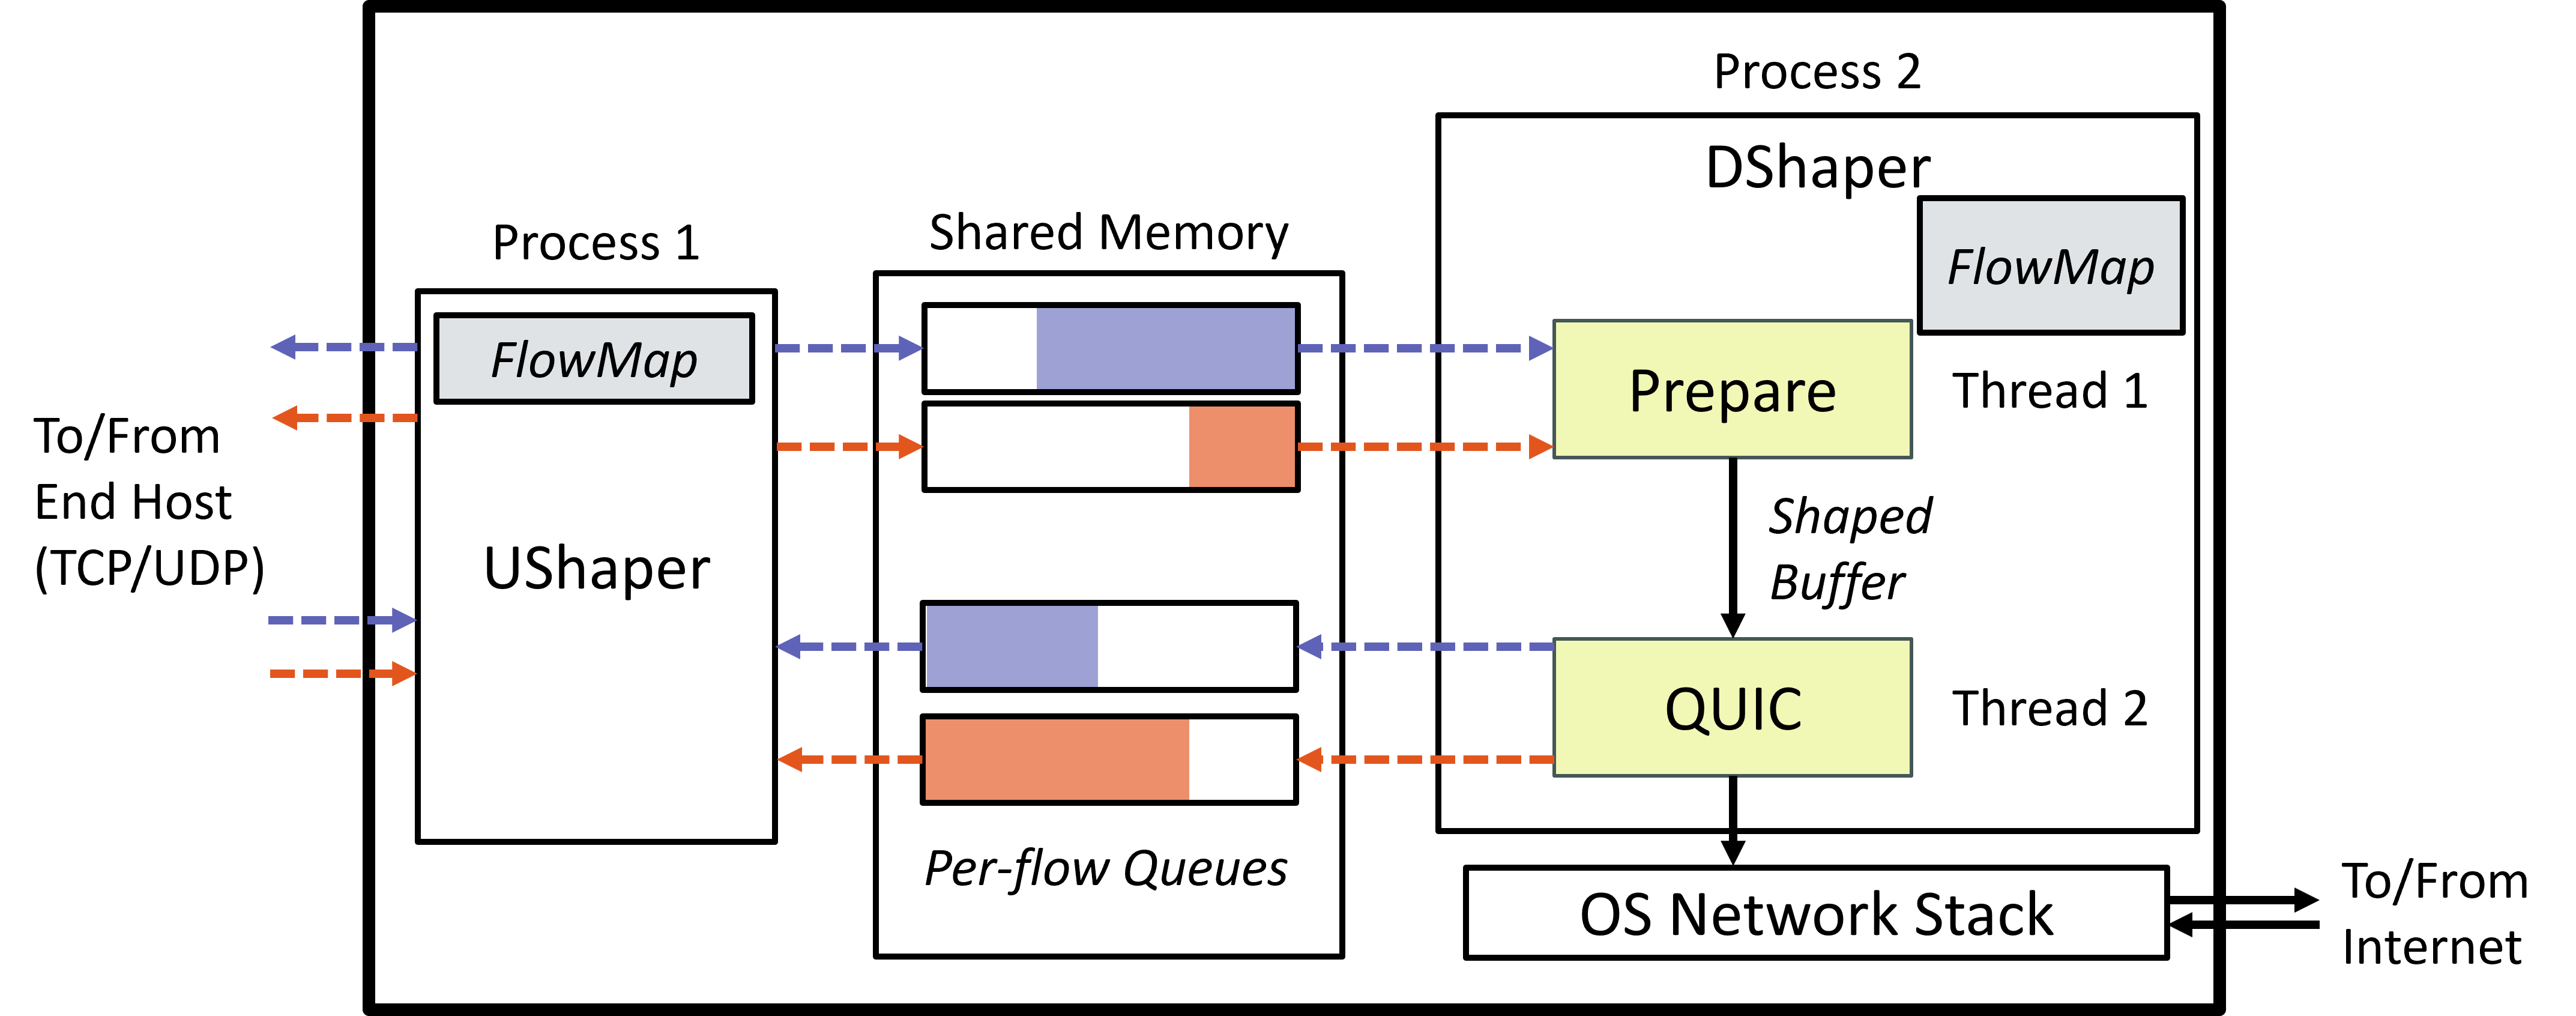
\includegraphics[width=\columnwidth]{figures/netshaper/middlebox-implementation.png}
    \caption{NetShaper Middlebox Implementation}
    \label{fig:middlebox-implementation}
\end{figure}

As outlined in \Cref{fig:middlebox-implementation}, NetShaper's middlebox consists of two main processes: UShaper and DShaper, and a shared memory between them.

\paragraph{Shared Memory.}
Both \textit{UShaper} and \textit{DShaper} have a shared memory between them.
The shared memory consists of $2*(k + 2)$ Lamport Queues (LQs) [??]
\footnote{Lamport Queues are lock-free single producer single consumer (SPSC) queues. They are useful to ensure that no locking is required when putting data in or pulling data out from the queues.}, 
where $k$ is the fixed number of streams that were configured at initialisation.
There is one queue for each direction of transmission for each of the $k$ streams that are initialised, and for the dummy and control streams.

Similar to the stream types outlined in \Cref{sec:netshaper-designing-traffic-shaping-tunnel}, \textit{Control} LQ transmits the information about a connection establishment or termination by an end host application. 
\textit{Dummy} LQ consists of dummy data that is received from or sent to the tunnel.
\textit{Data} LQ consists of the application byte stream that has been received from or has to be sent to the remote application.


\paragraph{UShaper.}
The \textit{UShaper} implements a client or a server to communicate with the end host.
The UShaper also consists of a FlowMap that maps an end-host application with a corresponding pair of LQs.
\textit{UShaper} updates the FlowMap whenever an end-host application establishes or terminates a connection and a \textit{control} message is generated and either sent or received on the \textit{control} LQ.
In addition, it assigns an unused pair of LQs (one outbound and one inbound) to a new client and revokes that whenever the client terminates the connection.
The \textit{UShaper} receives outbound traffic from the end host and enqueues the payload in the assigned LQ.
Similarly, it dequeues inbound traffic from the inbound LQs and sends it to the corresponding end hosts.

\paragraph{DShaper.}
The \textit{DShaper} consists of two threads: \textit{Prepare} and \textit{QUIC worker}, and a FlowMap.
The FlowMap maps an LQ with a pre-initialised QUIC stream.
The \textit{Prepare} thread also measures the data available in the outbound LQs at the start of the window $W$.
It then adds noise to this available size based on the DP parameters.
Finally, it enqueues the payload and padding that needs to be transmitted.
The \textit{QUIC worker} transmits the enqueued data out to the network.
It also processes the received data, places it in the relevant LQ, and updates the FlowMap whenever a client initialises or terminates a connection.

\subsection{Ensuring secret-independent shaping}
\label{subsed:netshaper-secret-independent-shaping-implementation}

In order to enforce DP guarantees, \textit{DShaper} needs to transmit $L + \eta$ bytes in every finite interval $W$.
In order to achieve this, \textit{DShaper} should satisfy the following properties.
\textbf{P1}: The \textit{prepare} thread should calculate $L + \eta$, prepare a buffer of that size, and enqueue that buffer for the \textit{quic worker} to transmit within $W$.
\textbf{P2}: The \textit{quic worker} should encrypt the packets from the buffer and forward them to the UDP stack, such that the total size of the payload prepared in $W$ is $L + \eta$.
\textbf{P3}: The UDP stack should transmit the encrypted packets within $W$.
Thanks to the post-processing property of DP, it suffices to only ensure P1, and \textbf{P4.} that the QUIC worker prepares the QUIC packets independently of the secret data.

However, there are some challenges in satisfying P1 and P4.
As both \textit{Prepare} and \textit{UShaper} deal with secret-dependent data, their execution time may affect the observable network behaviour, which in turn may lead to exposed secrets.
While the end host application is isolated from the middlebox, its flow control may be secret dependent and can affect the execution time of the \textit{prepare} thread.
For example, the presence or absence of an application's traffic can affect the time it takes for the \textit{prepare} thread to prepare the buffers.
If the \textit{quic worker} starts transmitting immediately, the secret dependent information may be visible in the network behaviour. 
This would also break P4, as the \textit{quic worker} prepares the QUIC packets based on the secret-dependent flow control.
NetShaper addresses this by ensuring that the \textit{prepare} thread takes a fixed amount of time ($T_{prep}$) to prepare the shaped buffer.
In addition, it also locks the buffer while it is being enqueued to the \textit{quic worker}, to ensure that the \textit{quic worker} does not start preparing the packets and transmitting immediately.
\textit{prepare} releases the lock after a fixed amount of time $T_{enq}$.
This ensures that the \textit{quic worker} only receives the shaped buffer at regular intervals of time.
We empirically profile the time taken by \textit{prepare} for $T_{prep}$ and $T_{enq}$ for buffers of various lengths and set the values to the maximum observed, with an additional margin on top.
We have outlined pseudo-code for both prepare and QUIC worker in \Cref{lst:prepare_and_worker}.


To ensure further isolation, \textit{prepare} and \textit{quic worker} threads are run on separate physical CPU cores.
\textit{UShaper} runs on a yet different CPU core, to ensure that the sending and receiving of unshaped, secret-dependent data does not affect the execution time of either of the \textit{DShaper} threads.
We assume that the time QUIC takes to encrypt and decrypt the shaped buffer does not have any correlation with the content of the buffer and only correlates with the size of the buffer (which is already shaped).



\begin{minipage}{\textwidth}
\lstinputlisting[language=Python]{code/netshaper/prepare_and_worker.py}
\captionsetup{type=lstlisting}
\caption{Prepare and QUIC Worker Pseudo-code}
\label{lst:prepare_and_worker}
\end{minipage}

\endinput

----------------------------------------------------------------
\begin{figure}[!htb]
    \centering
    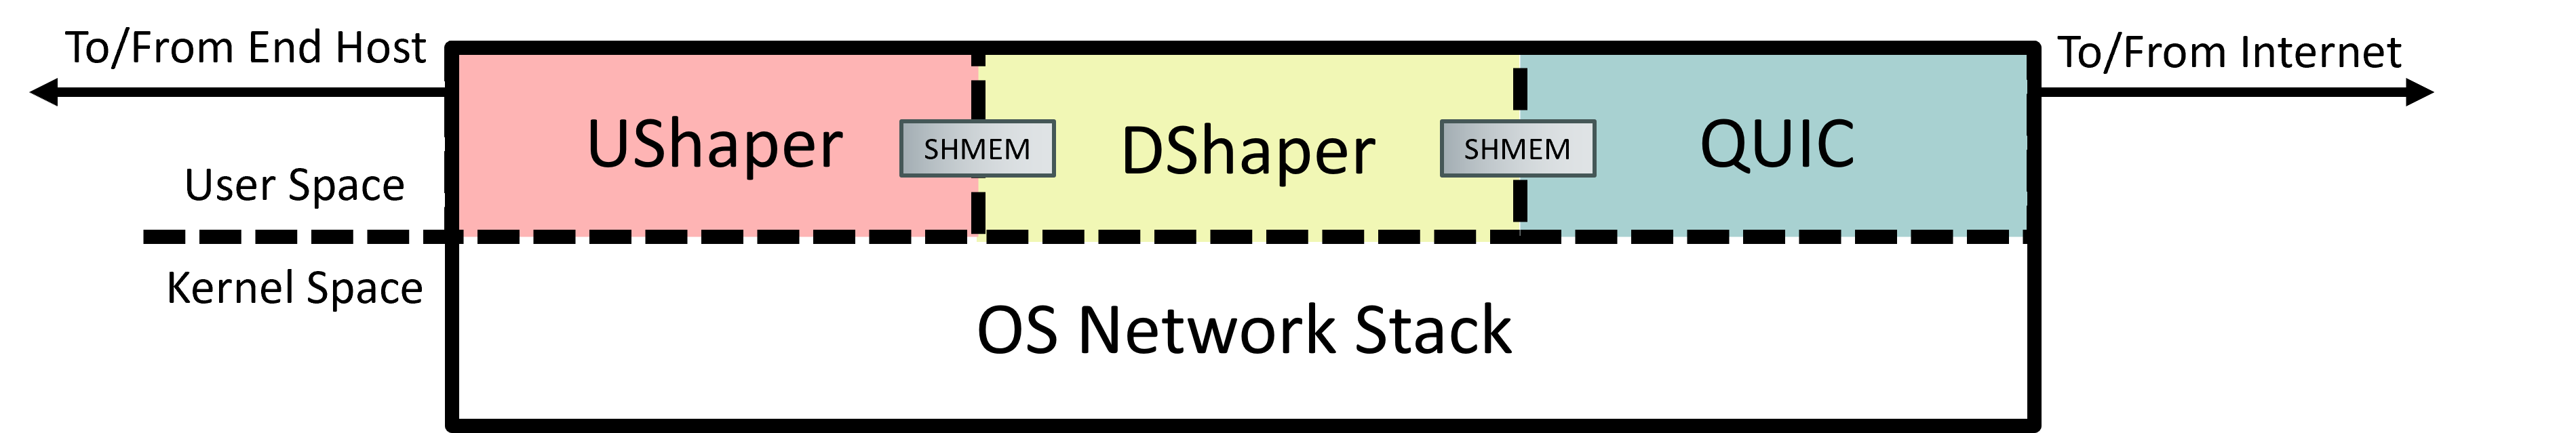
\includegraphics[width=\columnwidth]{figures/netshaper/middlebox-design-overview.png}
    \caption{Overview of NetShaper's Middlebox}
    \label{fig:middlebox-design-overview}
\end{figure}


-----------------------------------------------------------------
Should we add pseudo-codes for UShaper and DShaper?